\documentclass[UTF8,fontset=fandol,a4paper,10pt]{ctexart}
\usepackage[margin=18mm,top=16mm,bottom=17mm]{geometry}
\usepackage{amsmath,amssymb,graphicx,array}
\newcommand{\toprule}{\hline\noalign{\vskip 3pt}}
\newcommand{\midrule}{\noalign{\vskip 3pt}\hline\noalign{\vskip 3pt}}
\newcommand{\bottomrule}{\noalign{\vskip 3pt}\hline}
\usepackage[hidelinks]{hyperref}
\setlength{\parindent}{2em}
\setlength{\parskip}{3pt}
\linespread{1.13}
\ctexset{section={format=\large\bfseries,beforeskip=9pt,afterskip=4pt},subsection={format=\normalsize\bfseries,beforeskip=6pt,afterskip=2pt}}
\pagestyle{plain}
\newcommand{\src}[1]{{\footnotesize\noindent 数据来源：\texttt{#1}\par}}
\begin{document}
\begin{center}
{\LARGE\bfseries 两层哈希语义检索：算法设计与实验}\par
\vspace{4pt} {\small Exact Hash + 随机超平面 LSH \quad 算法设计实验报告 \quad 2026-10-26}
\end{center}

\section{问题、数据与表示}
给定历史问题库 $D=\{x_i\}_{i=1}^{N}$，既要快速识别原文重复，也要找回措辞不同但语义相近的问题。主实验 $N=10\,000$，以归一化向量的余弦阈值定义相关集合
\[
 G(q)=\{i:\widehat q^{\mathsf T}\widehat x_i\ge\tau\},\qquad \tau=0.75.
\]
这里的 Ground Truth 来自逐条暴力余弦计算，而非 Quora 原始配对标签；原配对只用于组织查询与校准阈值。

\textbf{数据。}使用 \texttt{sentence-transformers/quora-duplicates} 的 pair/train，原始 149,263 对；anchor 全字符串去重后有 86,169 条（重复比例 42.27\%）。基础库取 10,000 条唯一 anchor。验证集为 50 条语义查询与 10 条原文查询，测试集为 100 条语义查询与 20 条原文查询。验证与测试文本分离，语义查询原文排除在语料库之外；没有按检索得分删除难例。

\textbf{Embedding。}采用 \texttt{all-MiniLM-L6-v2}，CPU 编码，384 维，归一化后存为 float32；相似度计算重新归一化到 float64，并裁剪数值到 $[-1,1]$。最大已存向量范数误差为 $1.19\times10^{-7}$；判定直接使用 $s\ge\tau$，不添加容差。随机种子固定为 42。

\section{两层索引的设计与代价}
\textbf{第一层：Exact Hash。}用 Python 字典将完整原文映射到文档 ID 列表，哈希桶查找后按完整字符串相等确认；不做空格删除、大小写或 Unicode 归一化。普通哈希碰撞必须消解，避免把不同原文误认为相同。它能直接返回重复原文，却不能靠字符串相等发现改写问题。

\textbf{第二层：随机超平面 LSH。}每张表独立抽取 $k$ 个标准正态超平面，符号位 $h_j(x)=\mathbf1[a_j^{\mathsf T}\widehat x\ge0]$ 打包成一个整数签名（第 $j$ 位权重 $2^j$）；用 $L$ 个“签名 $\to$ ID 列表”的字典存储。查询只合并同签名桶，集合去重并排序，再对候选逐条余弦精筛。LSH 刻意增加相似向量的碰撞机会，碰撞本身不是最终相关性判定。系统没有全库兜底或 Ground Truth 注入。

\textbf{复杂度。}令 $d$ 为维数，$B$ 为命中桶的 ID 引用总数，$c=|C|$ 为去重候选数。LSH 建库时间 $O(NLkd)$，查询期望时间
\[
 O(Lkd+B+c\log c+cd),
\]
分别对应签名、桶合并、稳定排序、候选精筛。额外索引空间 $O(Lkd+NL)$，归一化工作矩阵另占 $O(Nd)$；候选向量临时空间为 $O(cd)$。Exact 对长度为 $\ell$ 的文本，平均桶定位 $O(1)$，连同哈希及 $m$ 个命中验证约 $O(\ell+m\ell)$，最坏碰撞可达 $O(N\ell+m\ell)$。原文总字符数为 $T$ 时建表约 $O(T+N)$。

\vfill
{\footnotesize\noindent 可复现版本：数据 revision \texttt{41f699770310302022a4dd75d4cf903bfef9ea46}；模型 revision \texttt{1110a243fdf4706b3f48f1d95db1a4f5529b4d41}。代码、配置与原始结果随项目保留。}

\newpage
\section{核心算法与参数依据}
\noindent\textbf{建库与查询伪代码}\par
\begin{quote}\small\ttfamily
Build(texts, X, k, L, seed):\\
\hspace*{1em}Exact[text].append(id); normalize X\\
\hspace*{1em}draw independent planes A[1..L, 1..k, 1..d]\\
\hspace*{1em}for each table t and document i:\\
\hspace*{2em}Buckets[t][pack(sign(A[t] X[i]))].append(i)\\[3pt]
Search(text, query):\\
\hspace*{1em}E = Exact.lookup\_and\_verify(text)\\
\hspace*{1em}if E is not empty: return E\quad // skip embedding and LSH\\
\hspace*{1em}q = normalize(query); C = empty set\\
\hspace*{1em}for t = 1..L: C.update(Buckets[t][signature(q)])\\
\hspace*{1em}R = empty list\\
\hspace*{1em}for i in sorted(C):\\
\hspace*{2em}if cosine(q, X[i]) >= tau: R.append(i)\\
\hspace*{1em}return R
\end{quote}
Exact 命中只返回原文 ID，不保证找齐所有超过余弦阈值的相关项；只有进入 LSH 的查询才满足 $R=C\cap G$。该路径中，候选召回与精筛后的 Recall 相同，精筛不会补回未进桶的相关项。

\textbf{碰撞概率推导。}对余弦相似度 $s$，单个随机超平面同号概率为 $p(s)$；一张表要求 $k$ 位全同，多表取并集，故
\[
 p(s)=1-\frac{\arccos s}{\pi},\qquad
 P(s;k,L)=1-\bigl(1-p(s)^k\bigr)^L.
\]
在 $s_1=0.75$，$p=0.76995$，$p^{12}=0.04340$；$L=16,32$ 时，$P$ 分别为 0.50835、0.75828。$s_0=0$ 时，$(k,L)=(12,32)$ 的 $P=0.007783$。若要求边界理论概率至少 0.9，则 $k=12$ 需 $L\ge52$。最终选型未达到该边界理论目标；验证平均 Recall 超过 0.9，不能据此宣称边界概率达标。

\textbf{先选 $\tau$，再选 $k,L$。}预先规定原配对覆盖率至少 90\%、随机非来源参考对超阈值率至多 1\%，取满足者中最高阈值。$\tau=0.70,0.75,0.80$ 的来源查询覆盖率分别为 49/50、46/50、38/50；5,000 个随机参考对在三阈值下均未超阈值（它们不是真实负标签）。因此先固定 $\tau=0.75$。

验证网格 $k\in\{8,12,16\},L\in\{4,8,16,32\}$，限定平均候选率 $\le5\%$、P95 $\le10\%$、LSH 索引 $\le32$ MiB，优先最大化条件 Recall。选得 $k=12,L=32$：验证 Recall 91.82\%，平均候选率 1.4702\%、P95 1.9385\%，LSH 索引 22.705 MiB。50 条语义验证查询中 48 条 $G$ 非空。配置于测试前冻结，测试未参与选型。

\section{统一评测口径}
Recall 为 $|R\cap G|/|G|$，只在 $|G|>0$ 的查询上取均值，空集数另报；Candidate Ratio 为精筛前 $|C|/N$。Query Cost 同时报查询耗时和实际余弦比较次数；Memory Cost 只计额外索引。MiB 均为 $2^{20}$ 字节。测试环境为 Windows 11、Python 3.12.6、NumPy 2.5.4。所有方法使用同一预计算 Embedding：预热 2 轮、重复 5 次、单线程，查询与方法交错执行。计时覆盖公开检索 API，不含下载、编码、加载、建库、Ground Truth 或内存扫描。

\newpage
\section{三方法实测与参数权衡}
主测试含 100 条语义查询，95 条 $G$ 非空，5 条空集全部保留；Recall 的分母样本量为 95，其余均值使用全部 100 条。表中额外索引不计共享文本、原始向量与归一化矩阵。
\begin{center}\small
\begin{tabular}{lrrrrr}\toprule
方法 & Recall(\%) & 候选率(\%) & 均时(ms) & 比较次数 & 索引(MiB)\\\midrule
Brute-force & 100.00 & 100.0000 & 1.9896 & 10000.00 & 0.000 \\
Exact-only & 0.00 & 0.0000 & 0.0025 & 0.00 & 1.381 \\
Hash + LSH & 96.77 & 1.5307 & 0.5451 & 153.07 & 24.079 \\
\bottomrule

\end{tabular}
\end{center}
\src{results/raw/method\_summary.csv（semantic 组）}
Hash + LSH 相对 Brute-force 的本次平均查询加速为 $3.65$ 倍，余弦比较减少 $98.47\%$，代价是约 $3.23$ 个百分点的 Recall 损失及 24.079 MiB 索引。Exact-only 的低耗时伴随语义 Recall 为零，不解决语义检索任务。三方法 P95 耗时依次为 2.6992、0.0034、0.7988 ms；Hybrid 的 P50 为 0.4873 ms，候选率 P95 为 2.2005\%。

\textbf{空间与建库。}Brute-force、Exact-only、Hybrid 的建库分别为 0.0416、0.00224、0.5941 s（前者包含归一化）。Hybrid 额外索引包含 Exact 与 LSH，不能与仅 LSH 的验证内存直接等同。使用去重后的 Python 对象深层大小估算，覆盖超平面、桶、键与 ID 引用，排除共享原文，不是 RSS 或峰值内存。原始 float32 向量为 15.36 MB；每个向量检索器的 float64 工作矩阵另占 30.72 MB。

\begin{center}
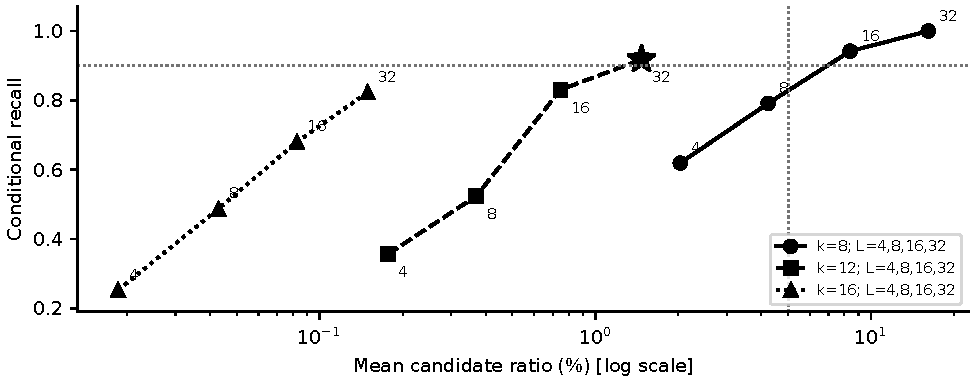
\includegraphics[width=.96\linewidth]{figures/recall_candidate.pdf}
\par\small 图 1：验证集 Recall 与候选率；点旁数字为 $L$，星号为冻结配置。
\end{center}
\src{results/raw/validation\_grid.csv（全部 12 组）}
图中虚线对应平均候选率 5\% 与 Recall 0.9；完整可行性还受 P95 与内存约束。固定 $k=12$，$L$ 从 4 增至 32，验证 Recall 从 35.62\% 升到 91.82\%，候选率从 0.1768\% 增至 1.4702\%。$k=8,L=16/32$ 虽有更高 Recall，但超候选预算；$k=16,L=32$ 的 Recall 为 82.37\%，索引 38.409 MiB，超过内存预算。参数调节是在召回、比较次数与存储间作取舍。

\textbf{Exact 子组与混合查询。}20 条原文测试全部精确命中，Hybrid 不做余弦比较，但按完整 $G$ 评测时 Recall 仅 82.08\%。例如一条原文查询有 4 个阈值相关项，捷径只返回原文 1 项，Recall 为 $1/4$。Exact 命中率 100\% 不等于语义 Recall 100\%。合并 120 条查询后，115 条 $G$ 非空；Hybrid Recall 为 94.21\%，均时 0.4600 ms。因查询组成不同，该值不能替代纯语义组的 96.77\%。

\newpage
\section{规模关系、局限与最后思考}
\textbf{真实规模实验。}固定相同 100 条语义查询、模型、$\tau,k,L$ 和同一组超平面，依次测量嵌套的 10k、50k、100k 语料。原 10k 及其向量逐字节保留；扩展从原始配对两列的去重并集抽样并排除语义查询原文。基础库只含 anchor，而扩展含两列，分布差异是解释结果的限制。
\begin{center}\small
\begin{tabular}{rrrrrr}\toprule
$N$ & Recall(\%) & 平均 $|C|$ & 平均 $|C\setminus G|$ & 均时(ms) & 索引(MiB)\\\midrule
10,000 & 96.77 & 153.07 & 151.20 & 0.402 & 24.079 \\
50,000 & 95.51 & 761.41 & 756.09 & 1.565 & 76.187 \\
100,000 & 93.65 & 1524.16 & 1514.93 & 2.557 & 139.005 \\
\bottomrule

\end{tabular}
\end{center}
\src{results/raw/scale\_summary.csv（独立规模运行）}
\begin{center}
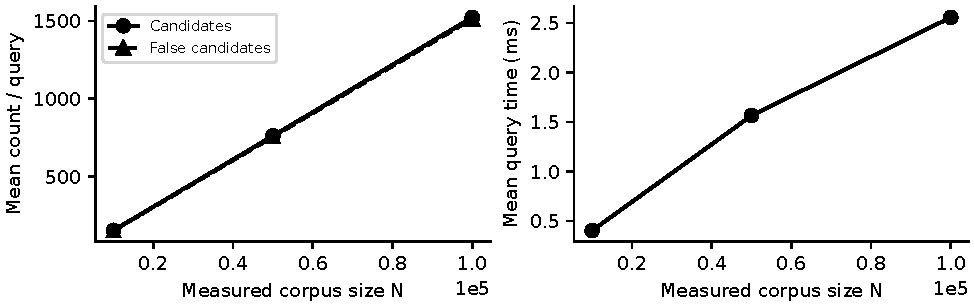
\includegraphics[width=.96\linewidth]{figures/scale.pdf}
\par\small 图 2：仅展示三个真实规模的候选数和查询时间，不含百万规模预测。
\end{center}
候选率约稳定在 1.52\%，但 $N$ 放大 10 倍，候选数扩大 9.96 倍，无关候选扩大 10.02 倍。最大桶从 48 增至 360。单表签名数最多 $2^{12}$，桶键数逐渐饱和，而 ID 引用仍随 $NL$ 增长，解释了索引增长低于 10 倍。10k 此次均时与主测试不同，来自独立测量，未覆盖主测试结果。

三个规模非空 $G$ 查询数为 95、98、98。扩大语料后 $C$ 与 $G$ 都可增长，但新增相关项不一定入桶，故 Recall 不保证单调上升；非空查询集合改变也影响条件均值。$|C\setminus G|$ 是随后被精筛丢弃的无关候选，不能称为最终误报。

\textbf{条件理论与外推，非实测。}对每条非相关向量 $i$，有
\[
 \mathbb E[F_q]=\sum_{i\notin G(q)}P(s_i;k,L)\approx NP_{\rm false}.
\]
固定参数不会自动随 $N$ 降低单对碰撞概率。若背景统一为 $s_0=0$，10k、100k、1m 的期望无关候选约为 77.83、778.30、7,783.01；若 $s_0=0.2$，则为 326.89、3,268.88、32,688.75。这是背景相似度假设下的理论计算，不是置信区间。沿用 10k 实测候选率对百万规模外推，平均候选约 15,307、无关候选约 15,120，同样\textbf{没有实测}。源数据不足百万条唯一问题，且百万 float32 原向量与 float64 工作矩阵已需 1.536+3.072 GB，故未强行运行。

\textbf{可能改进（未实现、未测量）。}小概率时 $\mathbb E[F]\approx NLp_0^k$；若 $p_0=0.5$，抵消十倍规模需约增加 $\log_2 10=3.32$ 位，即约 4 位，但会损失召回，补增 $L$ 又增加空间。大桶二次分裂或多探测也须重新验证召回与成本，不能直接宣称有效。

\textbf{最后思考。}Embedding 定义表示与相似性，不能自动解决海量检索。Exact 利用原文重复，LSH 用概率性候选削减计算，两者都需结合任务定义审视召回。实验表明候选比例小并不代表绝对候选数小；参数必须随规模和资源重新权衡。可靠结论还依赖独立验证、完整真值、统一计时与如实报告失败和外推边界。
\end{document}
